\documentclass[journal]{IEEEtran}

% Shared preamble: keep identical across both papers in this repository.
\usepackage[T1]{fontenc}
\usepackage{microtype}
\usepackage{amsmath,amssymb}
\usepackage{booktabs,tabularx,array,multirow}
\usepackage{graphicx}
\usepackage[dvipsnames]{xcolor}
\usepackage{cite}
\usepackage{url}
\usepackage[hidelinks]{hyperref}
\usepackage[nameinlink,capitalise]{cleveref}

\crefname{figure}{Fig.}{Figs.}
\Crefname{figure}{Fig.}{Figs.}
\crefname{table}{Table}{Tables}
\Crefname{table}{Table}{Tables}
\crefname{section}{Section}{Sections}
\Crefname{section}{Section}{Sections}
\crefname{subsection}{Section}{Sections}
\Crefname{subsection}{Section}{Sections}
\crefformat{equation}{(#2#1#3)}
\Crefformat{equation}{Equation~(#2#1#3)}
\crefrangeformat{equation}{(#3#1#4)--(#5#2#6)}

\newtheorem{definition}{Definition}
\newtheorem{proposition}{Proposition}
\newtheorem{corollary}{Corollary}
\crefname{definition}{Definition}{Definitions}
\crefname{proposition}{Proposition}{Propositions}
\crefname{corollary}{Corollary}{Corollaries}

\newcolumntype{Y}{>{\raggedright\arraybackslash}X}
\newcolumntype{P}[1]{>{\raggedright\arraybackslash}p{#1}}
\newcommand{\true}{\textsc{true}}
\newcommand{\false}{\textsc{false}}
\newcommand{\unknown}{\textsc{unknown}}

% Paper-specific packages.
\usepackage{tikz}
\usetikzlibrary{arrows.meta,positioning,calc}
\hyphenation{multi-robot middle-ware time-stamp}

\hypersetup{
  pdftitle={Contracts Across the Multi-Robot Execution Stack: A Cross-Layer Review and Reference Framework},
  pdfauthor={Mohammed Adil Farooq},
  pdfkeywords={multi-robot systems, assume-guarantee contracts, runtime assurance, runtime verification, ROS 2, age of information}
}

\begin{document}

\title{Contracts Across the Multi-Robot Execution Stack:\\
  A Cross-Layer Review and Reference Framework}

\author{Mohammed~Adil~Farooq%
\thanks{e-mail: \href{mailto:mdadilfarooq@gmail.com}{mdadilfarooq@gmail.com}}}

\maketitle

\begin{abstract}
Multi-robot systems connect mission planning to physical action through
software, communication, and runtime safety mechanisms.  Existing contract and
assurance techniques address different parts of this path, so information needed
to judge an upstream result may be lost before another component or robot uses
it.  This paper presents a focused survey of contract-based and
runtime-assurance approaches relevant to multi-robot execution.  I organize the
literature into six areas of concern: mission intent, component behavior,
dynamical interaction, distributed state, runtime authority, and embodied
execution.  I compare each class's mechanism, evidence, and scope.  Five
integration gaps recur within the reviewed corpus: semantic and physical
validity; temporal validity of distributed state; uncertainty, provenance, and
evidence; implementation and lifecycle compatibility; and intervention and
recovery authority.  I synthesize these observations into an edge-contract
reference framework.  It distinguishes interfaces within a robot from those
between robots and associates an admitted transfer with a typed payload,
assumptions, guarantees, validators, evidence, and recovery behavior.  A failure
taxonomy separately records fault origin, first observation, downstream effect,
and recovery authority.  The framework unifies obligations drawn from the
survey; it is neither a new contract calculus nor a validated reliability
mechanism.
\end{abstract}

\begin{IEEEkeywords}
Multi-robot systems, contract-based design, assume--guarantee reasoning,
distributed execution, runtime verification, runtime assurance.
\end{IEEEkeywords}

\section{Introduction}
\label{sec:introduction}

\IEEEPARstart{M}{ulti-robot} systems are assembled from components whose
correctness claims rest on different assumptions.  A mission synthesizer may
guarantee a temporal goal within a declared context; a planner may report
feasibility for a particular state and model; a learned predictor may forecast
peer motion over a horizon; middleware may report a quality-of-service event;
and a safety filter may guarantee forward invariance under a dynamics and timing
model.  Mission success depends on each claim and on whether its assumptions
still hold when another component, or another robot, consumes its output.  The
practical requirement is easy to state: \emph{a result should cross an
interface with enough context for the receiver to decide whether it is still
valid.}

This requirement is becoming harder to meet.  Multi-robot stacks now combine
classical task allocation and motion coordination
\cite{gerkey2004mrta,choi2009cbba,sharon2015cbs} with language-conditioned
planning and learned prediction \cite{mandi2024roco,obata2025lipllm,li2026llmmrs}.
Learned components expand capability, but they do not remove the need for
explicit physical, temporal, and deployment assumptions.  Inference is also
distributed: a prediction may be computed on board, next to the controller that
uses it, or remotely on infrastructure that fuses more data at the cost of
latency \cite{kehoe2015cloud}.  Each placement changes the interfaces that a
result must cross.  At lower layers, ROS~2 and the Data Distribution Service
(DDS) transport state and commands, while runtime-assurance and barrier-based
controllers may override a nominal decision before actuation
\cite{macenski2022ros2,omg2015dds,desai2019soter,wang2017barrier}.  An
end-to-end execution argument must therefore cross semantic, physical,
software, communication, and safety boundaries.

Multi-robot coupling makes this more than an ordinary integration problem.
Stale or ambiguous state at robot $r_i$ can make a locally admissible decision
invalidate robot $r_j$'s route, resource claim, or safety margin.  Join, leave,
restart, and partition events can invalidate assignments even when every message
is syntactically well formed.  The relevant interfaces are \emph{vertical},
between functions within one robot, and \emph{horizontal}, between robots or
distributed services (\cref{fig:command-path}).

\begin{figure}[htbp]
  \centering
  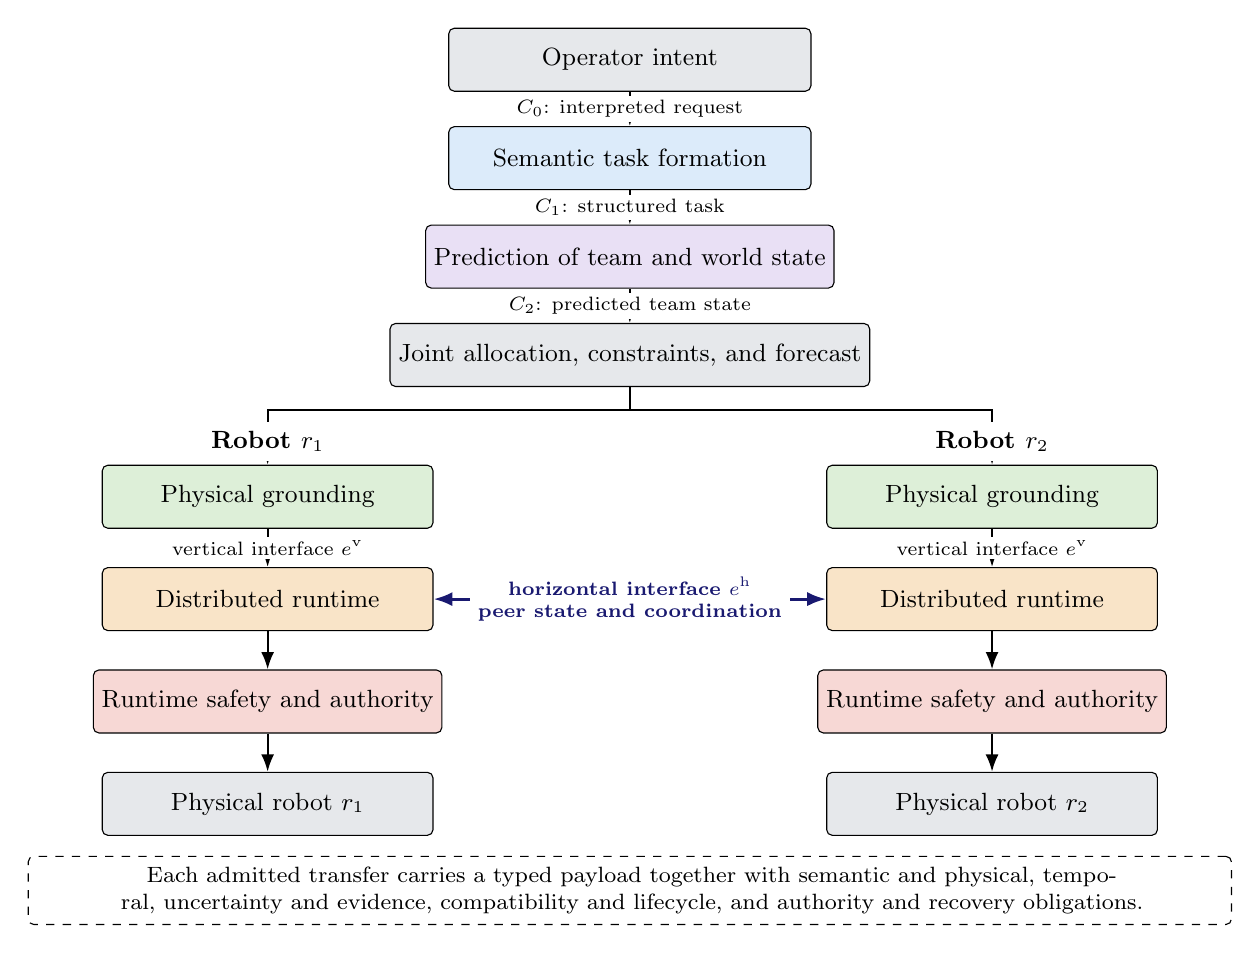
\begin{tikzpicture}[
    x=1cm,y=1cm,
    stage/.style={draw,rounded corners=2pt,minimum height=8mm,
      minimum width=46mm,align=center,font=\small,inner sep=3pt},
    lane/.style={stage,minimum width=42mm},
    flow/.style={-{Latex[length=2.2mm]},line width=0.8pt},
    peer/.style={{Latex[length=2.4mm]}-{Latex[length=2.4mm]},line width=1.1pt,
      draw=MidnightBlue},
    tag/.style={midway,fill=white,inner xsep=3pt,inner ysep=1.5pt,
      font=\scriptsize,align=center}
  ]
    \definecolor{IntentGray}{HTML}{E6E8EB}
    \definecolor{SemanticBlue}{HTML}{DCEBFA}
    \definecolor{PredictPurple}{HTML}{E9E0F5}
    \definecolor{PhysicsGreen}{HTML}{DDEFD8}
    \definecolor{RuntimeOrange}{HTML}{F9E4C8}
    \definecolor{SafetyRed}{HTML}{F7D8D5}

    \node[stage,fill=IntentGray] (intent) at (0,0) {Operator intent};
    \node[stage,fill=SemanticBlue] (task) at (0,-1.25)
      {Semantic task formation};
    \node[stage,fill=PredictPurple] (predict) at (0,-2.50)
      {Prediction of team and world state};
    \node[stage,fill=IntentGray] (joint) at (0,-3.75)
      {Joint allocation, constraints, and forecast};

    \draw[flow] (intent) -- node[tag] {$C_0$: interpreted request} (task);
    \draw[flow] (task) -- node[tag] {$C_1$: structured task} (predict);
    \draw[flow] (predict) -- node[tag] {$C_2$: predicted team state} (joint);

    \foreach \side/\xpos/\idx in {L/-4.6/1,R/4.6/2} {
      \node[lane,fill=PhysicsGreen] (ground\side) at (\xpos,-5.55)
        {Physical grounding};
      \node[lane,fill=RuntimeOrange] (runtime\side) at (\xpos,-6.85)
        {Distributed runtime};
      \node[lane,fill=SafetyRed] (safety\side) at (\xpos,-8.15)
        {Runtime safety and authority};
      \node[lane,fill=IntentGray] (robot\side) at (\xpos,-9.45)
        {Physical robot $r_{\idx}$};
      \draw[flow] (ground\side) -- node[tag] {vertical interface
        $e^{\mathrm v}$} (runtime\side);
      \draw[flow] (runtime\side) -- (safety\side);
      \draw[flow] (safety\side) -- (robot\side);
    }

    \coordinate (split) at (0,-4.45);
    \draw[line width=0.8pt] (joint.south) -- (split);
    \draw[flow] (split) -| (groundL.north);
    \draw[flow] (split) -| (groundR.north);
    \node[font=\small\bfseries,fill=white,inner xsep=3pt] at (-4.6,-4.85)
      {Robot $r_1$};
    \node[font=\small\bfseries,fill=white,inner xsep=3pt] at (4.6,-4.85)
      {Robot $r_2$};

    \draw[peer] (runtimeL.east) -- node[tag,text=MidnightBlue,
      font=\scriptsize\bfseries] {horizontal interface $e^{\mathrm h}$\\
      peer state and coordination} (runtimeR.west);

    \node[draw,dashed,rounded corners=2pt,align=center,font=\footnotesize,
      inner sep=4pt,text width=150mm] at (0,-10.55)
      {Each admitted transfer carries a typed payload together with semantic
       and physical, temporal, uncertainty and evidence, compatibility and
       lifecycle, and authority and recovery obligations.};
  \end{tikzpicture}
  \caption{Cross-layer command path of a two-robot team.  Single-headed arrows
  are producer--consumer transfers; $C_0$--$C_2$ label the shared
  command-formulation interfaces.  Vertical interfaces connect functions within
  one robot, and the double-headed horizontal interface exchanges peer state and
  coordination obligations between robots.}
  \label{fig:command-path}
\end{figure}


Existing work addresses parts of this problem through contract-based mission
design, quantitative mission assurance, component contracts for the Robot
Operating System (ROS), compositional reasoning for interconnected dynamics,
runtime monitoring, and safety-controller switching
\cite{mallozzi2020crome,chaki2013assurance,luckcuck2026compositional,
sharf2021dynamical,ghaffari2024rosmonitoring,desai2019soter}.  These approaches
protect different objects and produce different kinds of evidence.  This paper
asks whether their combined coverage supports the full multi-robot
command-to-action path:
\begin{enumerate}[\IEEEsetlabelwidth{RQ3:}]
  \item[RQ1:] Which objects, assumptions, and guarantees do existing
    contract-based and runtime-assurance approaches represent?
  \item[RQ2:] How are these claims composed, monitored, enforced, or repaired,
    and what evidence supports them?
  \item[RQ3:] Which obligations remain implicit when information crosses
    semantic, physical, distributed, and inter-robot boundaries, and what must
    an interface carry to make them checkable?
\end{enumerate}

The paper makes four contributions:
\begin{enumerate}
  \item a cross-layer taxonomy of contract-based and runtime-assurance
    approaches, organized by protected object, mechanism, and reported evidence
    (\cref{sec:taxonomy});
  \item a coverage analysis that identifies five recurring interface gaps,
    supported by a qualitative coverage matrix and by public failure reports
    from ROS~2 middleware (\cref{sec:gaps});
  \item an interface-contract reference framework with three-valued admission
    and recovery semantics, including a temporal admission margin for peer
    state that determines which metadata a horizontal interface must carry and
    when on-board inference is preferable to remote inference
    (\cref{sec:framework}); and
  \item a failure-attribution taxonomy and a worked command trace that assign
    validators and recovery authority along the command path
    (\cref{sec:attribution,sec:trace}).
\end{enumerate}

The framework is a reference model.  It does not define a new contract algebra,
and it has not been evaluated as a reliability mechanism.
\Cref{sec:background} states the interface problem, \cref{sec:method} describes
the review method, \cref{sec:taxonomy} presents the taxonomy, and
\cref{sec:gaps} derives the gaps.  \Cref{sec:framework} develops the
framework, \cref{sec:discussion} discusses its implications and limitations,
and \cref{sec:conclusion} concludes.

\section{The Multi-Robot Interface Problem}
\label{sec:background}

\subsection{Coupled Execution}

A multi-robot system contains a team $\mathcal R=\{r_1,\ldots,r_n\}$ whose
objectives, observations, actions, or resources are coupled
\cite{gerkey2004mrta,street2023formal,gielis2022communications}.  The coupling
may arise from a shared mission, collision
constraints, task precedence, limited resources, or communication through a
time-varying graph.  Consequently, local correctness is generally insufficient:
a decision that is safe for one robot under an old peer state can violate the
joint constraint under the current team state.

Let $x_i$, $u_i$, and $w_i$ denote the state, input, and disturbance of robot
$i$.  A general model is
\begin{equation}
  \dot x_i=f_i(x_i,u_i,w_i),
  \qquad
  g_{ij}(x_i,x_j)\ge 0,\qquad \{i,j\}\in\mathcal E_c,
  \label{eq:coupled-dynamics}
\end{equation}
where $\mathcal E_c$ indexes coupled team constraints.  For collision avoidance,
for example, $g_{ij}=\lVert p_i-p_j\rVert^2-d_{\min}^2$; other instances encode
formation, visibility, or other coupled state constraints
\cite{sharf2021dynamical,chen2019invariance,wang2017barrier}.  The local dynamics
in \cref{eq:coupled-dynamics} can be valid while the joint constraint is evaluated
with an invalid peer state.  This is the mechanical reason that horizontal
interfaces require explicit timing and uncertainty assumptions.

A typical command passes through task interpretation, allocation, prediction,
motion or action planning, distributed communication, runtime validation, and
physical execution.  These functions need not occupy separate processes or
robots, but each transformation changes the object being reasoned about.  A
language instruction becomes a task model; a task model becomes an assignment;
an assignment becomes trajectories or actions; and distributed observations
become inputs to safety-critical control.  Evidence that is meaningful at one
stage may be insufficient at the next.

\subsection{What a Contract Protects}

An assume--guarantee contract separates an environment assumption $A$ from a
component guarantee $G$ \cite{benveniste2007contracts}.  A contract theory may
also define satisfaction, compatibility, refinement, composition, and quotient
for a chosen behavioral model.  Robotics uses this idea at several levels: a
mission contract can describe temporal goals and contexts; a component contract
can specify software behavior; a dynamical contract can constrain input and
output trajectories; and a runtime-assurance specification can govern transfer
of control authority.  These contract objects are related, but they are not
interchangeable.

Here, a \emph{contract} states obligations, \emph{verification} checks a stated
property, and \emph{assurance} is the broader argument and evidence supporting
confidence in system behavior.  A contract contributes to assurance only when
its assumptions, checking mechanism, and evidence are explicit.

This distinction matters because an interface schema is not automatically a
contract.  Names, types, timestamps, and version fields become contractual only
when they participate in explicit assumptions or guarantees, are checked by a
defined validator, and have a specified consequence when the check fails.
Likewise, a runtime monitor observes only the properties encoded in its
specification; it cannot infer an omitted frame, validity horizon, or recovery
policy.  The survey therefore considers both the stated property and the
evidence used to support it.

\subsection{Evidence Boundary}

Because every guarantee depends on its assumptions, the type of supporting
evidence matters.  The survey distinguishes three forms.  \emph{Capability evidence}
shows that a system performs a task.  \emph{Assurance evidence} supports a
specified property under declared assumptions, for example through proof,
synthesis, monitoring, or testing.  \emph{Deployment evidence} measures behavior
on a stated platform, configuration, workload, or fault condition.  A planning
benchmark is therefore not evidence of network-timing robustness, and a formal
guarantee under a dynamics model is not evidence that an implementation uses
the correct frame, clock, or software version.  The survey compares approaches
within their reported evidence boundaries and does not treat all successful
demonstrations as equivalent.  This distinction is especially important for
coordinated-autonomy studies, where a mission-level probability or reliability
estimate can be valid for its model and data without certifying every runtime
interface used to execute the mission
\cite{chaki2013probabilistic,porter2013reliability}.

\section{Review Method}
\label{sec:method}

We conducted a structured narrative review of how contract-based and
runtime-assurance approaches represent, compose, monitor, enforce, or repair
assumptions that cross robot-software and inter-robot interfaces.  Each source
was examined with four questions:
\begin{enumerate}
  \item What is the primary object of reasoning: mission, component behavior,
    dynamical interaction, distributed state, runtime authority, or embodied
    execution?
  \item Which mechanism does the source supply: specification, refinement,
    composition, synthesis, monitoring, testing, intervention, or repair?
  \item Which kind of evidence does it report (\cref{sec:evidence-kinds}), and
    does that evidence include a physical multi-robot system?
  \item Which semantic, physical, temporal, uncertainty, evidence,
    compatibility, lifecycle, and authority obligations does it leave to
    adjacent components?
\end{enumerate}

\emph{Search.}  We searched arXiv and web-indexed IEEE, ACM, Springer, Elsevier,
and institutional repositories by title, abstract, and full text.  Core queries
combined \emph{assume--guarantee} or \emph{contract-based} with \emph{robot},
\emph{ROS}, \emph{multi-robot}, \emph{multi-agent}, \emph{mission
specification}, \emph{coordinated autonomy}, \emph{mission reliability},
\emph{probabilistic model checking}, \emph{runtime verification}, and
\emph{runtime assurance}.  Backward and forward snowballing from foundational
contract work, coordinated-mission assurance, robotic mission frameworks, ROS
contract and monitoring systems, and recent cross-layer reviews added sources
that use different terminology.

\emph{Selection.}  We included primary work that defines a contract,
compositional-assurance, runtime-monitoring, or runtime-assurance mechanism
applicable to robotics, cyber-physical systems, or interconnected agents;
reports a relevant robotics implementation; or defines a directly relevant
communication standard.  We also included surveys that organize multi-robot
modeling, communication, learning, safety, or embodied assurance.  We excluded
general design-by-contract work without an architectural or cyber-physical
connection and planning work that does not expose an interface-assurance
question.  Representative planning and middleware sources were retained only
where they clarify what an interface must carry.

\emph{Coding.}  For each source, we recorded the protected object, mechanism,
reported evidence, deployment setting, and obligations left to adjacent
components, and we grouped sources into twelve approach classes under six
protected objects (\cref{tab:taxonomy}).  The coded corpus contains 36 sources.
The remaining 15 references supply background on multi-robot coordination and
middleware, foundational contract theory, the standards used by the framework,
related surveys, and the public issue reports analyzed in
\cref{sec:middleware-evidence}.  Coverage of each obligation is coded per class
(\cref{tab:coverage}).  A class receives ``E'' when the obligation is explicit
and central in every source of the class, ``P'' when the treatment is partial,
conditional, model-internal, or present in only some sources, and ``--'' when
the obligation lies outside the stated mechanisms.  The coding describes the
cited mechanisms, not every capability of the surrounding systems.

\emph{Scope of inference.}  The search evolved through snowballing, so
PRISMA-style candidate and exclusion counts were not retained.  The review
therefore supports qualitative statements about coverage and evidence
boundaries; it supports no claim about prevalence or effect size.

\section{Contract-Based and Runtime Assurance by Protected Object}
\label{sec:taxonomy}

We organize the reviewed literature by its \emph{protected object}: the
property or artifact that an approach is designed to preserve.
\Cref{tab:taxonomy} summarizes the twelve approach classes; the classes overlap,
and one system can contribute to more than one of them.

\begingroup
\footnotesize
\setlength{\tabcolsep}{3pt}
\renewcommand{\arraystretch}{1.08}
\begin{longtable}{@{}P{0.15\textwidth}P{0.15\textwidth}P{0.21\textwidth}P{0.21\textwidth}P{\dimexpr0.28\textwidth-24pt\relax}@{}}
  \caption{Reviewed approaches grouped by what they protect}
  \label{tab:taxonomy}\\
  \toprule
  Approach class & Protected object & Mechanism & Reported evidence & Obligations left to adjacent components \\
  \midrule
  \endfirsthead
  \multicolumn{5}{@{}l}{\textit{Table \thetable{} continued}}\\
  \toprule
  Approach class & Protected object & Mechanism & Reported evidence & Obligations left to adjacent components \\
  \midrule
  \endhead
  \midrule
  \multicolumn{5}{r@{}}{\textit{Continued on next page}}\\
  \endfoot
  \bottomrule
  \endlastfoot
    \multicolumn{5}{@{}l}{\textit{Mission intent}} \\*
    Mission contracts \cite{mallozzi2020crome,mallozzi2023contextual,mallozzi2023repair}
      & Goals, contexts, and component libraries
      & Contract-based goal graphs, refinement, synthesis, context switching, and repair
      & Mission examples and synthesized controllers; no physical team evaluation
      & Physical validity, event-time state, implementation identity, and peer reconciliation \\
    Language-conditioned planning \cite{mandi2024roco,obata2025lipllm}
      & Instructions, roles, task dependencies, and plans
      & Dialogue with environment feedback; dependency graph with a linear program
      & Multi-robot benchmarks, simulation, and selected real-world execution
      & Calibrated uncertainty, timing, compatibility, and deployment assurance \\
    Coordinated-mission assurance \cite{chaki2013assurance,chaki2013probabilistic,porter2013reliability,stancliff2006missionreliability}
      & Mission phases, coordination, utility, and team reliability
      & Markov-chain model checking, probabilistic verification, and reliability estimation
      & In-progress robot validation, measured robot behavior, and repairable-team analysis
      & Interface-carried uncertainty, provenance, software identity, lifecycle state, and recovery evidence \\
    \addlinespace[2pt]
    \multicolumn{5}{@{}l}{\textit{Component behavior}} \\*
    Component contracts and monitors \cite{luckcuck2026compositional,ghaffari2024rosmonitoring,caldas2024rvft}
      & ROS node assumptions, guarantees, and message traces
      & First-order contracts, composition rules, and generated monitors; topic and service monitoring; testing guidelines
      & Inspection-rover and smaller examples; UAV case study; literature, repository, and practitioner studies
      & Team epoch, resource ownership, state age, and evidence lineage \\
    Distributed programming and design \cite{ghosh2020koord,harbin2023design}
      & Coordination programs, proof obligations, and team architecture
      & Executable semantics, modular verification, generated infrastructure, and simulation-based robustness analysis
      & Three Koord applications; three simulated ATLAS case studies
      & Runtime freshness, evidence lineage, heterogeneous implementation identity, and recovery authority \\
    \addlinespace[2pt]
    \multicolumn{5}{@{}l}{\textit{Dynamical interaction}} \\*
    Dynamical contracts \cite{sharf2021dynamical,chen2019invariance,liu2022stlcontracts}
      & Input/output trajectories, invariant sets, and temporal tasks
      & Satisfaction and refinement checks, compositional invariance, and decentralized synthesis
      & Two-vehicle, microgrid, and numerical simulations
      & Message age, lifecycle, implementation identity, and recovery semantics \\
    Assume--guarantee learning \cite{kazemi2024agrl}
      & Neighbor abstractions, labels, and local policies
      & Regular-language contracts with a lower bound on global satisfaction probability
      & Grid-world, room-temperature, and traffic-signal case studies
      & Physical and middleware validity of the assumed abstractions \\
    \addlinespace[2pt]
    \multicolumn{5}{@{}l}{\textit{Distributed state}} \\*
    Middleware and QoS \cite{macenski2022ros2,omg2015dds,maruyama2016ros2,kronauer2021latency}
      & Data streams, delivery status, and endpoint compatibility
      & QoS policies and offered/requested matching; end-to-end latency measurement across DDS implementations
      & Standard and architecture descriptions; configuration-specific benchmarks
      & Event-time validity, physical decision validity, evidence lineage, and recovery \\
    Communication-aware coordination \cite{gielis2022communications,silva2026probabilistic,kaul2012aoi}
      & Information freshness and intermittent connectivity
      & Age-of-information analysis; temporal communication constraints in stochastic multi-robot planning
      & Critical review; analytical results; planning simulations
      & Implementation identity, evidence lineage, and coordinated recovery \\
    \addlinespace[2pt]
    \multicolumn{5}{@{}l}{\textit{Runtime authority}} \\*
    Runtime assurance and safety filters \cite{sha2001simplex,desai2019soter,shivakumar2020soterros,ames2017cbf,wang2017barrier,garg2024safecontrol}
      & Safety properties, safe sets, and control authority
      & Controller switching, barrier-constrained inputs, and learned safe control with verification
      & Drone surveillance in simulation and hardware; simulated multi-robot surveillance; wheeled-robot experiments; survey
      & Semantic evidence, implementation compatibility, and upstream reporting of interventions \\
    Mission-level runtime verification \cite{tsai2026missionrta,kekatos2026swarmrta}
      & Mission feasibility and swarm-level policies
      & Pre-execution command rejection; compositional verdicts with an explicit unknown
      & Simulated driving fault scenarios; simulated swarm mission
      & Physical feasibility, implementation identity, and recovery orchestration \\
    \addlinespace[2pt]
    \multicolumn{5}{@{}l}{\textit{Embodied execution}} \\*
    Cross-layer guardrails and runtimes \cite{kim2026guardrails,liu2026phyagentos,kim2026safeembodied}
      & Layered interventions, execution sessions, and evidence
      & Monitoring and intervention layers; compatibility preflight, session verification, and heartbeat
      & Position paper; simulated and physical embodiments; structured review
      & Common composition semantics across peer-robot interfaces \\
\end{longtable}
\endgroup


\subsection{Related Surveys}

Recent surveys use other organizing lenses.  Li \emph{et al.}\ classify
language-model research for multi-robot systems into task allocation, motion
planning, action generation, and human intervention \cite{li2026llmmrs}.
Street \emph{et al.}\ review formal models for robot teams under uncertainty,
and Gielis \emph{et al.}\ analyze how robotic applications and communication
systems interact \cite{street2023formal,gielis2022communications}.  Garg
\emph{et al.}\ organize learning-based safe control by safety notion, control
method, and verification tool \cite{garg2024safecontrol}.  Kim \emph{et al.}\
review safety for long-horizon manipulation by intervention locus (planning,
policy, and execution) and grade the strength of the supporting evidence
\cite{kim2026safeembodied}.  These surveys clarify capabilities, models,
communication, or intervention layers.  The present review uses a different
unit of comparison: the protected object, together with the information required
when its guarantee becomes another component's assumption.

\subsection{Mission Intent}

CROME captures mission requirements as contract-based goal graphs, checks
feasibility, refines goals from a library, and synthesizes controllers
\cite{mallozzi2020crome}; later work decomposes contextual missions into
context-specific sub-missions with correct-by-construction switching
\cite{mallozzi2023contextual}.  Contract operations can also refine a mission
against a component library or repair an unrealizable specification
\cite{mallozzi2023repair}.  These methods make goals, contexts, refinement, and
realizability explicit at the mission boundary; data age, provenance, and
implementation identity lie outside their scope.

Language-conditioned planners address an adjacent problem: turning open-ended
instructions into plans, role assignments, or optimization models.  RoCo
coordinates language-model agents through dialogue with environment feedback,
and LiP-LLM combines a language model with a predefined skill set, a dependency
graph, and a linear program \cite{mandi2024roco,obata2025lipllm}.  Both provide
capability evidence, while collision checking, skill definitions, and
feasibility solvers remain external.  Expressing intent is not the same as
certifying its physical or distributed execution.

Quantitative assurance of coordinated autonomy addresses the mission level from
another direction.  Chaki, Dolan, and Giampapa characterize coordination
phenomena and mission phases and evaluate discrete-time Markov-chain models by
probabilistic model checking \cite{chaki2013assurance}; related work computes
mission utility by probabilistic verification \cite{chaki2013probabilistic}.
Reliability studies estimate the performance of sequentially coordinated
missions from measured robot behavior and compare repairable team
configurations \cite{porter2013reliability,stancliff2006missionreliability}.
Within the reviewed corpus, this line is the closest mission-level predecessor
of the present question because it connects coordination structure to
quantitative mission evidence.  Its protected object is mission or team
reliability, whereas we ask which obligations must cross the heterogeneous
interfaces that realize such a mission.

\subsection{Component Behavior}

Luckcuck \emph{et al.}\ specify ROS nodes with first-order assume--guarantee
contracts, compose node contracts into system properties through inference
rules, and translate contracts written in the ROS Contract Language (RCL) into
executable runtime monitors \cite{luckcuck2026compositional}.  The approach
connects behavioral contracts to node implementations; cross-robot state age,
team membership, and heterogeneous deployment compatibility are not its central
objects.  ROSMonitoring~2.0 monitors topics and services, including message
order, with partial ROS~2 support \cite{ghaffari2024rosmonitoring}.  Caldas
\emph{et al.}\ contribute guidelines for runtime verification and field-based
testing of ROS-based systems that emphasize observability, instrumentation, and
reporting \cite{caldas2024rvft}.  Together, these works show that
specification, instrumentation, and evidence collection are separate
engineering concerns.

Distributed robot programming and model-driven design connect software
structure to team behavior more directly.  Koord provides platform-independent
abstractions for distributed shared memory, sensing, and control; its executable
semantics expose proof obligations, of which platform-specific ones are checked
with physics-based models and hybrid verification tools \cite{ghosh2020koord}.
ATLAS models team architecture, mission, and collective intelligence and uses
simulation to explore design choices and robustness \cite{harbin2023design}.
Both analyses remain tied to their languages, models, generated infrastructure,
and simulation settings; neither defines an evidence envelope for every
interface of a heterogeneous deployed stack.

\subsection{Dynamical Interaction}

Contracts for dynamical systems place assumptions on input trajectories and
guarantees on outputs.  Sharf \emph{et al.}\ verify satisfaction and refinement
of linear contracts by linear programming and prove safety in a two-vehicle
example \cite{sharf2021dynamical}.  Chen \emph{et al.}\ use parameterized
temporal-logic contracts to compute robust invariant sets compositionally for
network systems \cite{chen2019invariance}, and Liu \emph{et al.}\ synthesize
decentralized controllers for interconnected nonlinear systems from
signal-temporal-logic contracts \cite{liu2022stlcontracts}.  Assume--guarantee
reinforcement learning expresses contracts over neighboring components as
regular languages and combines local satisfaction probabilities into a lower
bound for the whole system \cite{kazemi2024agrl}.  These approaches address
interaction and decomposition directly, but they assume that the declared
neighbor abstractions, labels, communication, dynamics, and timing are available
as modeled.

\subsection{Distributed State}

ROS~2 provides modular robot communication through interchangeable middleware
implementations, most commonly DDS \cite{macenski2022ros2,omg2015dds}.  DDS
quality-of-service (QoS) policies govern reliability,
history, durability, liveliness, deadline, and lifespan.  These are
data-stream mechanisms; they do not establish application-level freshness or
mission validity.  The \emph{Deadline} policy concerns the expected period
between samples, not the age of the physical event a sample represents.  The
\emph{Lifespan} policy expires samples relative to their source time stamp,
which by default records the write call rather than the physical event; the
standard relies on sufficiently synchronized clocks and allows a reader to
substitute the reception time stamp when it detects that they are not
\cite{omg2015dds}.

ROS~2 latency studies show that process structure, executor behavior, and the
DDS implementation affect end-to-end timing
\cite{maruyama2016ros2,kronauer2021latency}.  Communication surveys find that
coordination and networking assumptions are often designed and evaluated
separately \cite{gielis2022communications}, and recent planning work builds
temporal communication constraints and intermittent connectivity into
stochastic multi-robot planning \cite{silva2026probabilistic}.  Age-of-information
research characterizes how fresh the newest available update is
\cite{kaul2012aoi}.  These works provide deployment semantics and measurements
rather than compositional robot contracts.  They nevertheless expose a necessary
bridge: a dynamical or safety guarantee that assumes current peer state needs an
application-level rule that relates event time, clock uncertainty, delivery, and
the physical decision.

\subsection{Runtime Authority}

The Simplex architecture uses a simple, verified controller to bound the
behavior of a more complex one \cite{sha2001simplex}.  SOTER makes this pattern
programmable for robotics: a decision module transfers authority from an
advanced controller to a safe controller when a monitor predicts a violation
\cite{desai2019soter}, and SOTER on ROS evaluates the pattern in simulated
multi-robot surveillance \cite{shivakumar2020soterros}.  Control barrier
functions and multi-robot barrier certificates instead constrain the admissible
inputs to keep a modeled safe set invariant \cite{ames2017cbf,wang2017barrier}.
These mechanisms give strong conditional safety guarantees, but the guarantees
depend on the dynamics model, state estimation, update rate, feasibility, and
timely peer state.  A local intervention can preserve one robot's safety while
invalidating the team plan unless it is reported upstream.

Mission-level runtime verification extends monitoring beyond immediate safety.
Tsai and Hariri reject driving commands that would make the mission infeasible
before they execute \cite{tsai2026missionrta}.  Kekatos \emph{et al.}\ compose
platform, squad, and mission monitors for robot swarms over a messaging fabric
that makes evidence loss observable, so that unsupported negative verdicts
become an explicit \emph{unknown} rather than an all-clear
\cite{kekatos2026swarmrta}.  This treatment of missing evidence is the closest
reviewed counterpart to the admission semantics of \cref{sec:admission}.

\subsection{Embodied Execution}

Kim \emph{et al.}\ argue for modular safety guardrails that monitor and
intervene across action, decision, and human-centered safety
\cite{kim2026guardrails}.  PhyAgentOS separates cognitive planning from physical
execution and provides compatibility preflight, supervised execution sessions,
evidence-grounded verification, layered safety, and heartbeat monitoring
\cite{liu2026phyagentos}.  It is the closest reviewed runtime architecture to
several obligations synthesized here.  PhyAgentOS, however, defines one
embodied-agent runtime, whereas the framework of \cref{sec:framework} is an
architecture-independent classification of obligations on both cross-layer and
peer-robot interfaces.  Within the reviewed works, we found no composition model
that jointly represents temporal validity, ownership, provenance, and recovery
across those interfaces.

\subsection{Synthesis}

The reviewed literature supplies mechanisms for mission realizability, node
behavior, dynamical composition, communication observation, and runtime safety.
Coverage becomes discontinuous where these mechanisms meet.  A mission guarantee
may end before physical feasibility; a dynamical guarantee may assume current
neighbor signals; a middleware status may omit the physical event time; and a
safety intervention may never return to task allocation.  \Cref{sec:gaps}
turns these discontinuities into five interface gaps.

\section{Cross-Layer Interface Gaps}
\label{sec:gaps}

The reviewed approaches use different behavioral models, so their guarantees
cannot be combined simply by listing them.  A cross-layer execution argument
must preserve the assumptions that matter when an output expressed under one
model becomes an input to another.  \Cref{tab:coverage} codes each approach
class against seven interface obligations, and four patterns stand out.  No
class is explicit and central on more than two of the seven obligations.  No
class treats membership, ownership, and lifecycle transitions as explicit and
central.  Temporal validity is explicit only in the two distributed-state
classes, which treat physical validity and recovery at most partially.  Recovery
is explicit only where authority transfer is local to one controller or one
runtime.  The obligations group into five recurring gaps, G1--G5.

\begin{table}[!t]
  \centering
  \caption{Qualitative Coverage of Interface Obligations by Approach Class}
  \label{tab:coverage}
  \footnotesize
  \setlength{\tabcolsep}{2.4pt}
  \newcommand{\colhead}[1]{\rotatebox{90}{#1}}
  \begin{tabular}{@{}>{\raggedright\arraybackslash}p{0.5\columnwidth}*{7}{c}@{}}
    \toprule
    & \multicolumn{2}{c}{G1} & G2 & G3 & \multicolumn{2}{c}{G4} & G5 \\
    \cmidrule(lr){2-3}\cmidrule(lr){4-4}\cmidrule(lr){5-5}\cmidrule(lr){6-7}\cmidrule(l){8-8}
    Approach class & \colhead{Semantic} & \colhead{Physical} & \colhead{Temporal}
      & \colhead{Uncertainty} & \colhead{Compatibility} & \colhead{Lifecycle}
      & \colhead{Recovery} \\
    \midrule
    Mission contracts                    & E  & P  & -- & -- & -- & P  & P  \\
    Language-conditioned planning        & E  & P  & -- & -- & -- & -- & P  \\
    Coordinated-mission assurance        & E  & P  & -- & E  & -- & P  & P  \\
    Component contracts and monitors     & P  & P  & P  & -- & P  & -- & P  \\
    Distributed programming and design   & E  & P  & P  & P  & E  & P  & P  \\
    Dynamical contracts                  & -- & E  & -- & -- & -- & -- & -- \\
    Assume--guarantee learning           & P  & P  & -- & E  & -- & -- & -- \\
    Middleware and QoS                   & -- & -- & E  & -- & E  & P  & -- \\
    Communication-aware coordination     & P  & P  & E  & P  & -- & P  & P  \\
    Runtime assurance and safety filters & -- & E  & P  & P  & -- & -- & E  \\
    Mission-level runtime verification   & E  & P  & P  & P  & -- & -- & P  \\
    Cross-layer guardrails and runtimes  & P  & E  & P  & P  & P  & P  & E  \\
    \bottomrule
  \end{tabular}

  \vspace{3pt}
  \parbox{\columnwidth}{\scriptsize E: explicit and central in every source of
  the class; P: partial, conditional, model-internal, or present in only some
  sources; --: outside the stated mechanisms.  Semantic: task identity, intent,
  and hard constraints.  Physical: feasibility or safety under a physical model.
  Temporal: event time, data age, validity interval, and clock semantics.
  Uncertainty: uncertainty representation, provenance, and evidence kind.
  Compatibility: implementation, version, and configuration identity.
  Lifecycle: membership, ownership, and lifecycle transitions.  Recovery:
  defined response to a failed check, including authority transfer.  G1--G5
  refer to the gaps of \cref{sec:gaps}; sources per class are listed in
  \cref{tab:taxonomy}.}
\end{table}


\subsection{G1: Semantic and Physical Validity}

Mission contracts make goals and contexts explicit, and planning and learning
systems produce assignments or actions.  The receiving component still needs the
task identifiers, capabilities, map, state, dynamics, resources, and
communication model behind a proposal.  It must also be able to distinguish a
hard constraint from a planner preference, a model suggestion, and a checked
feasibility claim.  A meaningful plan may be physically infeasible, and a
feasible plan may violate the operator's intent.  Feasibility must therefore be
qualified as nominal, robust, probabilistic, or conditional on a named model and
operating region
\cite{mallozzi2020crome,mallozzi2023repair,mandi2024roco,obata2025lipllm,
chaki2013probabilistic}.

\subsection{G2: Temporal Validity of Distributed State}
\label{sec:gap-time}

Distributed execution involves several distinct times: the time of the physical
event, the publication time, the arrival time, the time at which the consumer
can use the data, the target time of a forecast, and the end of the validity
interval.  Replacing the event time with a reception time stamp hides both
producer and network delay.  For a stream of state updates, the age of
information at time $t$ is
\begin{equation}
  \Delta(t)=t-u(t),
  \label{eq:aoi}
\end{equation}
where $u(t)$ is the event time of the newest update available to the consumer
\cite{kaul2012aoi}.  Age matters only relative to a decision: the same sample can
be fresh enough for a slow inspection task and too old for collision avoidance
between fast robots.  Comparing event times across robots also requires the
clocks to be comparable.  Synchronization protocols such as IEEE~1588 can bound
the offset between clocks \cite{ieee2020ptp}, but the bound helps the consumer
only if it travels with the time stamp.  Transport reliability or a cadence
notification does not establish that the margin a decision needs is available
\cite{omg2015dds,kronauer2021latency}.  A cross-robot interface therefore needs
event-time semantics, the clock domain and an error bound, an
application-specific validity bound, and a response to stale or incomparable
state.  \Cref{sec:temporal-admission} derives these fields from the collision
constraint in \eqref{eq:coupled-dynamics}.

\subsection{G3: Uncertainty, Provenance, and Evidence}

The word \emph{uncertainty} may refer to a covariance, an interval, a reachable
set, a calibrated probability, or semantic ambiguity.  These representations
cannot be compared or propagated in the same way, and a confidence value with no
declared meaning cannot satisfy a downstream chance constraint or robust margin.
The interface must identify the representation, the covered variables and
correlations, the calibration regime, the validity horizon, and the propagation
rule.

The same requirement applies to evidence.  A consumer should be able to tell a
proof from a solver status, a monitor verdict, a calibration report, a test
identifier, and a deployment measurement.  Provenance links a payload and its
evidence to the model, configuration, observations, and transformations that
produced them.  Without this lineage, a downstream rejection may reveal that a
claim failed but not which assumption or artifact needs repair
\cite{kim2026safeembodied,w3c2013prov}.

\subsection{G4: Implementation and Lifecycle Compatibility}

Type and wire compatibility are weaker than behavioral compatibility.  Two
components can decode the same message while using different coordinate frames,
units, parameter sets, middleware implementations, dependency versions, or clock
sources.  Admitting a result therefore requires separate identities for the
schema, protocol, implementation, dependencies, and configuration, together with
evidence that the combination is supported
\cite{macenski2022ros2,omg2015dds,kronauer2021latency}.

Message contracts also omit lifecycle unless it is represented explicitly.
Join, leave, restart, and partition recovery can invalidate old assignments or
duplicate resource ownership.  A multi-robot contract needs a team epoch,
membership and ownership state, legal lifecycle transitions, and a
reconciliation rule for retained or delayed data
\cite{luckcuck2026compositional,liu2026phyagentos}.

\subsection{G5: Intervention, Recovery, and Attribution}

Monitoring is incomplete if a failed check has no defined consequence.  The
responsible authority may request clarification, obtain fresh state,
re-estimate, replan, transfer control, degrade the mission, isolate a robot,
stop, or escalate to a human.  In a team, this response must be coordinated: an
unreported local safety override can invalidate peer trajectories or
task-completion logic.  Runtime-assurance and field-testing work accordingly
treats intervention, observability, and reporting as first-class mechanisms
\cite{desai2019soter,shivakumar2020soterros,caldas2024rvft}.

Fault origin and first observation must also be kept apart.  A collision risk
first detected by a controller may originate in semantic grounding, prediction,
physical modeling, communication delay, or hardware.  Recording origin, first
observation, effect, and recovery authority as separate fields supports both
online handling and post-mission diagnosis.

\subsection{Evidence from ROS~2 Middleware}
\label{sec:middleware-evidence}

Public failure reports from the nightly continuous-integration (CI) pipeline of
Nav2, the ROS~2 navigation stack, illustrate G2 and G4 in deployed software
\cite{nav2issue6163}.  Unchanged Nav2 test sources failed for different reasons
under three ROS middleware (RMW) implementations.
\begin{itemize}
  \item With \texttt{rmw\_zenoh}, the ROS~2 middleware based on Zenoh
    \cite{corsaro2023zenoh}, tests passed every assertion yet aborted at
    process exit: \texttt{rclcpp::shutdown()} ran from the destructor of a
    global test-fixture object after the thread-local storage of the Zenoh
    runtime had already been destroyed.  Moving initialization and shutdown
    into \texttt{main()} removed the failures \cite{nav2pr4948,nav2pr6241}.
  \item With Cyclone DDS, a teardown assertion in \texttt{ddsi\_fini} appeared
    with release~11.0.1 but not with 11.0.0, using the same
    \texttt{rmw\_cyclonedds\_cpp} version.  Reverting one upstream commit that
    changed the type-lookup request and reply headers eliminated the failure in
    40 repeated runs, although that commit may expose rather than contain the
    defect \cite{cyclonedds2426}.
  \item With Fast DDS, a service request reached its server and the callback
    ran, but the response was dropped because the response writer had not yet
    matched the client's response reader; increasing the client's wait time did
    not help.  The behavior is consistent with a known limitation of service
    discovery in the Fast DDS middleware layer
    \cite{nav2issue6163,fastrtps392}.
\end{itemize}

In each case, the message types, the application code, and the declared QoS
were unchanged.  What differed was the implementation identity, its patch
version, or the order of lifecycle events, which is exactly the information
that a type-level interface does not carry (G4).  The Fast DDS case also shows
that the availability of one endpoint is not evidence that a complete
request--response interaction can occur in time (G2).  The author contributed the
Zenoh fix and the Cyclone DDS diagnosis; all observations are taken from the
public record.  These are single-host test failures rather than multi-robot
field incidents, so they illustrate the gaps but do not measure their
prevalence.

\section{A proposed interface framework}
\label{sec:framework}

I use the five gaps to propose a common record for information passed between
components or robots.  The record states what is being sent, why the receiver
may use it, how to check it, and what to do if the check fails.  Formal claims
about refinement, realizability, controller synthesis, or the whole system
still need the appropriate behavioral models from \cref{sec:taxonomy}.

\begin{table}[htbp]
  \centering
  \caption{Interface-Contract Obligations Derived from the Five Gaps}
  \label{tab:obligations}
  \footnotesize
  \setlength{\tabcolsep}{3pt}
  \renewcommand{\arraystretch}{1.08}
  \begin{tabularx}{\textwidth}{@{}P{0.17\textwidth}P{0.33\textwidth}P{0.25\textwidth}Y@{}}
    \toprule
    Gap & Metadata and evidence carried by the interface & Required validators & Response on rejection \\
    \midrule
    G1: Semantic and physical validity
      & Canonical task and resource identifiers; hard constraints; frames and units; model, operating region, and margins
      & Registry resolution; task, feasibility, or certificate check
      & Clarify, reject, repair the task, or replan \\
    G2: Temporal validity
      & Event or forecast-target time; publication and availability times; validity interval; clock domain and error bound
      & Freshness, target-time, deadline, and clock-comparability predicates, e.g., \eqref{eq:temporal-admission}
      & Request fresh state, shorten the horizon, degrade, or stop \\
    G3: Uncertainty, provenance, and evidence
      & Uncertainty type, scope, correlations, calibration, and propagation rule; model and solver identity; lineage; evidence kind
      & Uncertainty-threshold, calibration, certificate, and provenance-policy checks
      & Re-estimate, re-solve, choose a robust alternative, or escalate \\
    G4: Implementation and lifecycle compatibility
      & Schema, protocol, implementation, dependency, and configuration identities; membership; resource ownership; team epoch
      & Supported-combination, epoch, ownership, and lifecycle-transition checks
      & Reconcile, downgrade, isolate, restart, or reallocate \\
    G5: Intervention, recovery, and attribution
      & Producer and consumer authority; safety overrides; acknowledgements; completion evidence; recovery owner
      & Authority, acknowledgement, intervention-report, and completion predicates
      & Transfer authority, coordinate replanning, stop, or request human action \\
    \bottomrule
  \end{tabularx}
\end{table}


\subsection{Interfaces as Producer--Consumer Edges}

I represent the deployed system as a directed graph whose vertices are
functions assigned to robots or services.  A \emph{vertical} edge
$e^{\mathrm v}=(r,k)\rightarrow(r,k+1)$ connects consecutive functions of robot
$r$, while a \emph{horizontal} edge $e^{\mathrm h}=(r,k)\rightarrow(s,l)$ with
$s\neq r$ connects robots or distributed services.  A horizontal edge is more
than another message path: its consumer may act on behalf of a different robot
and thereby change joint feasibility, resource ownership, or a peer's safety
margin.  Vertical edges usually share a clock, an implementation, and a
lifecycle; horizontal edges usually do not.

\subsection{Interface Contracts}

\begin{definition}[Interface contract]\label{def:interface-contract}
For an edge $e=(p,c)$ from producer $p$ to consumer $c$, an interface contract
is the tuple
\begin{equation}
  C_e=(P_e,M_e;\,A_e,G_e,V_e,E_e,R_e),
  \label{eq:contract}
\end{equation}
where $P_e$ is a typed payload; $M_e$ is typed metadata, such as identifiers,
frames and units, times, uncertainty semantics, implementation identities, team
epoch, and lineage; $A_e$ is the consumer's assumption; $G_e$ is the producer's
guarantee; $V_e$ is a set of validators or monitor references; $E_e$ is the
supporting evidence, such as a solver result, proof, calibration report, monitor
record, or test identifier; and $R_e$ is the response to rejection or unresolved
validity.
\end{definition}

A metadata field is contractual only when it appears in $A_e$, $G_e$, $V_e$, or
$R_e$.  \Cref{tab:obligations} maps each gap of \cref{sec:gaps} to the metadata,
validators, and recovery actions that an interface contract must specify; it is
the bridge from the review to the framework.  Provenance can reuse the
entity--activity--agent relations of W3C PROV \cite{w3c2013prov}.  The framework
keeps schema, protocol, and implementation identity separate because, as
\cref{sec:middleware-evidence} shows, syntactic compatibility does not establish
behavioral compatibility.

\subsection{Compatibility and Admission}
\label{sec:admission}

On a single edge, local compatibility requires the producer's guarantee to imply
the consumer's assumption:
\begin{equation}
  G_e\Longrightarrow A_e.
  \label{eq:compatibility}
\end{equation}
A consumer with several peer inputs must additionally check joint assumptions,
such as a common team epoch, consistent frames, unique resource ownership, and a
reconciliation rule after a partition; per-message checks cannot establish these
relations.  Condition \eqref{eq:compatibility} is therefore local.  Proving
that a composed team satisfies a global mission property requires defined
input--output ownership, feedback and temporal semantics, and a composition or
refinement calculus \cite{luckcuck2026compositional,mallozzi2023repair}.

Validators make the condition operational.  A syntactic validator checks
decoding, required fields, types, dimensions, units, frames, and schema
compatibility.  A semantic validator may call a solver, a runtime monitor, a
perception check, a calibrated statistical test, or a certificate verifier.
Each validator returns a value in $\{\true,\false,\unknown\}$.  Let
$\mathcal Q_e$ be the set of checks required on edge $e$, covering syntax,
time, uncertainty, compatibility, assumptions, guarantees, and provenance.
The edge admits the transfer at time $t$ if and only if every required check
returns \true:
\begin{equation}
  \operatorname{Admit}_e(t)\Leftrightarrow
  V_{e,q}(P_e,M_e,E_e,t)=\true\ \ \forall q\in\mathcal Q_e.
  \label{eq:admission}
\end{equation}
A required check that returns \unknown{} blocks admission, so missing metadata
or evidence leads to rejection rather than to silent acceptance; Kekatos
\emph{et al.}\ apply the same principle to missing monitoring evidence in robot
swarms \cite{kekatos2026swarmrta}.  Advisory checks outside $\mathcal Q_e$ may
return \unknown{} without blocking.  Condition \eqref{eq:admission} is what turns
descriptive fields into an enforced boundary: every required predicate takes
part in the execution decision.

\begin{table}[htbp]
  \centering
  \caption{Cross-Layer Failure-Attribution Taxonomy}
  \label{tab:attribution}
  \footnotesize
  \setlength{\tabcolsep}{3pt}
  \renewcommand{\arraystretch}{1.08}
  \begin{tabularx}{\textwidth}{@{}P{0.11\textwidth}P{0.15\textwidth}P{0.15\textwidth}YP{0.16\textwidth}P{0.15\textwidth}@{}}
    \toprule
    Origin & Local fault & Contract concern & First observation & Possible effect & Recovery authority \\
    \midrule
    Perception and estimation
      & Misassociation, bias, or clock error
      & Payload, frame, time, and uncertainty
      & Estimator innovation, semantic grounding, or controller residual
      & Wrong referent, localization drift, or unsafe state
      & Re-estimate, use a sensor fallback, or stop \\
    Semantic planning
      & Invented relation, capability, or priority
      & Intent, assumptions, and guarantees
      & Task-model validator or downstream feasibility check
      & Wrong or impossible assignment; repeated replanning
      & Clarify, repair, or replan \\
    Prediction
      & Biased or overconfident forecast
      & Horizon, uncertainty semantics, and validity evidence
      & Forecast residual or downstream feasibility check
      & Coordination failure or poor recovery
      & Re-estimate, shorten the horizon, or choose a robust plan \\
    Physical model
      & Missing constraint or inaccurate contact model
      & Feasibility claim and solver evidence
      & Optimizer status, controller residual, or contact event
      & Slip, saturation, collision, or damage
      & Re-optimize, switch to a fallback controller, or stop \\
    Runtime and network
      & Delay, loss, partition, version, or lifecycle fault
      & Age, clock, protocol, implementation identity, and assumptions
      & Consumer validator, missed update, exception, or teardown error
      & Inconsistent team state, abort, deadlock, or collision
      & Degrade, reconnect, reallocate, or restart \\
    Safety function
      & Local or unreported intervention
      & Authority, intervention evidence, and recovery
      & Safety monitor or upstream acknowledgement
      & Safe local motion but failed mission or new conflict
      & Coordinated replanning or human escalation \\
    Hardware
      & Sensor, actuator, energy, or compute fault
      & Capability and health guarantees
      & Health monitor, tracking residual, or peer timeout
      & Task abandonment or unsafe compensation by peers
      & Isolate the robot and reallocate its tasks \\
    \bottomrule
  \end{tabularx}
\end{table}


\subsection{Temporal Admission for Peer State}
\label{sec:temporal-admission}

The collision constraint of \eqref{eq:coupled-dynamics} shows which metadata a
horizontal interface must carry for a temporal validator to return \true.

\begin{proposition}[Temporal admission margin]
\label{prop:temporal-admission}
Let robots $r_i$ and $r_j$ have speeds bounded by $\bar v_i$ and $\bar v_j$, and
express all times in the consumer's clock.  Suppose the consumer holds position
estimates $\hat p_k$, $k\in\{i,j\}$, with stamped event times $\hat t_k$, such
that the true event time $t_k\le t$ satisfies $\lvert\hat t_k-t_k\rvert\le
\kappa_k$ and $\lVert\hat p_k-p_k(t_k)\rVert\le\varepsilon_k$.  For a decision
taken at time $t$ and held until $t+h$, let
$\bar\Delta_k=t+h-\hat t_k+\kappa_k$.  If
\begin{equation}
  \lVert\hat p_i-\hat p_j\rVert\ \ge\ d_{\min}
  +\sum_{k\in\{i,j\}}\bigl(\varepsilon_k+\bar v_k\bar\Delta_k\bigr),
  \label{eq:temporal-admission}
\end{equation}
then $\lVert p_i(s)-p_j(s)\rVert\ge d_{\min}$ for all $s\in[t,t+h]$.
\end{proposition}

\begin{proof}
Fix $s\in[t,t+h]$ and $k\in\{i,j\}$.  Because $t_k\le t\le s$ and
$t_k\ge\hat t_k-\kappa_k$, the true age satisfies
$0\le s-t_k\le\bar\Delta_k$.  The speed and error bounds give
$\lVert p_k(s)-\hat p_k\rVert\le\lVert p_k(s)-p_k(t_k)\rVert
+\lVert p_k(t_k)-\hat p_k\rVert\le\bar v_k\bar\Delta_k+\varepsilon_k$.  The
triangle inequality then yields $\lVert p_i(s)-p_j(s)\rVert\ge\lVert\hat
p_i-\hat p_j\rVert-\sum_k(\varepsilon_k+\bar v_k\bar\Delta_k)\ge d_{\min}$.
\end{proof}

Condition \eqref{eq:temporal-admission} is sufficient but not necessary, and it
is conservative because it ignores the direction of motion.  Its value here is
structural: every term on its right-hand side is a field that the interface must
carry or the consumer must already know.  The validator needs the event time
$\hat t_k$ rather than the reception time, the clock-error bound $\kappa_k$, an
error bound $\varepsilon_k$ with declared meaning, and the speed bound $\bar v_k$.
If any of these is missing, the validator returns \unknown{} and the decision is
not admitted.  Substituting the reception time for $\hat t_k$ understates the
age by the producer and network delay, which is exactly the failure described
in G2.

\begin{corollary}[Validity interval]\label{cor:validity-interval}
Under the assumptions of \cref{prop:temporal-admission}, let
$a_k=t-\hat t_k$ be the stamped age at decision time and
\[
  m(t)=\lVert\hat p_i-\hat p_j\rVert-d_{\min}
  -\sum_{k}\bigl(\varepsilon_k+\bar v_k(a_k+\kappa_k)\bigr)
\]
the separation margin that remains at that time.  Condition
\eqref{eq:temporal-admission} holds if and only if $h\le h^\star(t)$, where
\begin{equation}
  h^\star(t)=\frac{m(t)}{\bar v_i+\bar v_j}.
  \label{eq:validity-interval}
\end{equation}
\end{corollary}

\begin{proof}
Since $\bar\Delta_k=a_k+\kappa_k+h$, condition \eqref{eq:temporal-admission} is
equivalent to $m(t)\ge(\bar v_i+\bar v_j)\,h$, and $\bar v_i+\bar v_j>0$.
\end{proof}

If $h^\star(t)<0$, the pair cannot be admitted at time $t$ on these estimates.
Otherwise, the admitted state carries an explicit expiry time $t+h^\star(t)$,
after which the consumer must refresh it or invoke $R_e$.  The validity interval
that the gaps call for is thus computed by the consumer from fields carried on
the interface, not asserted by the producer.

\emph{Inference placement.}  \Cref{prop:temporal-admission} also prices the
choice between an on-board and a remote estimate of the same peer.  Suppose
robot $r_i$ can use either an on-board estimate of $p_j$, with error bound
$\varepsilon^{\mathrm L}$ and stamped age $a^{\mathrm L}=t-\hat t^{\mathrm L}$
on its own clock, or a remote estimate fused from more sensors, with error bound
$\varepsilon^{\mathrm R}$, stamped age $a^{\mathrm R}$, and clock-error bound
$\kappa^{\mathrm R}$.  The peer term in \eqref{eq:temporal-admission} is
$\varepsilon+\bar v_j(a+h+\kappa)$, so the on-board estimate consumes no more
of the separation margin than the remote one whenever
\begin{equation}
  \varepsilon^{\mathrm L}-\varepsilon^{\mathrm R}
  \ \le\ \bar v_j\bigl(a^{\mathrm R}+\kappa^{\mathrm R}-a^{\mathrm L}\bigr).
  \label{eq:placement}
\end{equation}
A remote estimate is worth its latency only if its accuracy advantage exceeds
the distance the peer can travel during the additional age and clock
uncertainty.  For example, with $\bar v_j=1.5$\,m/s, an additional
$120$\,ms of age, and a $10$\,ms clock-error bound, the remote estimate must be
at least $0.195$\,m more accurate.  The required advantage grows linearly with
peer speed, which is why on-board inference matters most for fast interactions,
whereas remote inference remains attractive for slow, wide-area decisions such
as task allocation \cite{kehoe2015cloud}.

\begin{table}[t]
  \centering
  \caption{Running command trace; all thresholds are scenario-specific contract parameters}
  \label{tab:command-trace}
  \scriptsize
  \begin{tabularx}{\textwidth}{@{}P{0.13\textwidth}P{0.27\textwidth}Y Y@{}}
    \toprule
    Function & Payload $P_e$ & Assumption, guarantee, and metadata & Validator and rejection $V_e,R_e$ \\
    \midrule
    Semantic task formation & Roles, sector identifier, inspection goal, and corridor-clear constraint & $A_e$: referents resolve and two capable robots exist; $G_e$: confirmed hard constraints remain explicit & Resolve against map and capability registries; clarify or reject an unresolved referent \\
    Predictive state & Occupancy and joint trajectories over horizon $H$ & $M_e$: event and target times, horizon, uncertainty semantics, and other-agent policy identity & Reject or shorten $H$ if age exceeds $\bar\Delta$ or uncertainty is not below its declared limit $\bar U$ \\
    Physical grounding & Reachable viewpoints and time-parameterized paths & $G_e$: separation is at least $d_{\min}$ and actuator limits hold; $E_e$: model, solver status, and minimum margins & Re-solve or return infeasible when solver status is unacceptable or a required margin is negative \\
    Distributed runtime & Assignments, paths, peer state, and acknowledgements & $M_e$: frame, units, schema/protocol/implementation identities, team epoch, ownership, and clock-error bound & Drop expired or wrong-epoch data; reconcile, degrade, or replan when age, clock, ownership, or compatibility checks fail \\
    Runtime safety & Admissible command or intervention record & $G_e$: conditional local-safety claim; $E_e$: active constraint, model/state/update assumptions, and intervention cause & Apply a feasible override and publish its cause; stop or escalate if the safety program is infeasible \\
    Physical robots & Execution state, health, resource release, and completion evidence & Capability and health guarantee; ownership and completion status & Isolate an unhealthy robot, reallocate its task, or request human action \\
    \bottomrule
  \end{tabularx}
\end{table}


\subsection{Recovery and Lineage}

A \false{} or a required \unknown{} invokes $R_e$: request clarification or
fresh data, re-estimate, replan, degrade, isolate, stop, or escalate.  The
rejection record names the failed predicate, the time, the evidence, and the
responsible interface.  A repaired result receives new lineage and does not
silently replace the rejected claim (\cref{fig:lifecycle}).

\begin{figure}[!t]
  \centering
  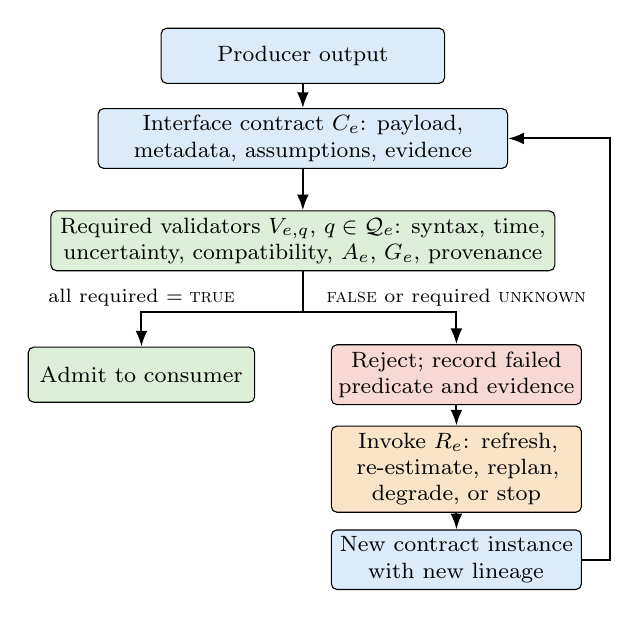
\begin{tikzpicture}[
    x=1cm,y=1cm,
    box/.style={draw,rounded corners=2pt,minimum height=7mm,align=center,
      font=\footnotesize,inner sep=2.5pt},
    arrow/.style={-{Latex[length=2mm]},line width=0.7pt},
    tag/.style={font=\scriptsize,align=center,inner sep=1pt}
  ]
    \definecolor{ContractBlue}{HTML}{DCEBFA}
    \definecolor{ValidatorGreen}{HTML}{DDEFD8}
    \definecolor{RecoveryOrange}{HTML}{F9E4C8}
    \definecolor{RejectRed}{HTML}{F7D8D5}

    \node[box,fill=ContractBlue,minimum width=36mm] (producer) at (0,0)
      {Producer output};
    \node[box,fill=ContractBlue,minimum width=52mm] (contract) at (0,-1.05)
      {Interface contract $C_e$: payload,\\metadata, assumptions, evidence};
    \node[box,fill=ValidatorGreen,minimum width=64mm] (validators) at (0,-2.35)
      {Required validators $V_{e,q}$, $q\in\mathcal Q_e$: syntax, time,\\
       uncertainty, compatibility, $A_e$, $G_e$, provenance};

    \coordinate (branch) at (0,-3.25);
    \node[box,fill=ValidatorGreen,text width=27mm] (admit) at (-2.05,-4.05)
      {Admit to consumer};
    \node[box,fill=RejectRed,text width=30mm] (reject) at (1.95,-4.05)
      {Reject; record failed predicate and evidence};
    \node[box,fill=RecoveryOrange,text width=30mm] (recover) at (1.95,-5.25)
      {Invoke $R_e$: refresh, re-estimate, replan, degrade, or stop};
    \node[box,fill=ContractBlue,text width=30mm] (repair) at (1.95,-6.40)
      {New contract instance with new lineage};

    \draw[arrow] (producer) -- (contract);
    \draw[arrow] (contract) -- (validators);
    \draw[line width=0.7pt] (validators.south) -- (branch);
    \draw[arrow] (branch) -| (admit.north);
    \draw[arrow] (branch) -| (reject.north);
    \node[tag,anchor=south] at (-2.05,-3.22) {all required $=\true$};
    \node[tag,anchor=south] at (1.95,-3.22) {\false{} or required \unknown};
    \draw[arrow] (reject) -- (recover);
    \draw[arrow] (recover) -- (repair);
    \draw[arrow] (repair.east) -- ++(0.35,0) |- (contract.east);
  \end{tikzpicture}
  \caption{Admission and recovery on one interface.  A required check that
  returns \unknown{} blocks admission like \false.  A successful repair creates a
  new contract instance and provenance record while preserving the rejected
  claim.}
  \label{fig:lifecycle}
\end{figure}


\subsection{Failure Attribution}
\label{sec:attribution}

The same physical outcome can have several origins.  A collision may begin with
an incorrect semantic relation, a biased prediction, a missing physical
constraint, stale peer state, or a hardware fault.  Conversely, downstream
checks can turn the same originating fault into a rejection, a degraded mission,
or a safe stop.  The taxonomy in \cref{tab:attribution} therefore records the
origin, the contract concern, the first observation, the effect, and the
recovery authority as separate fields; the first observation is the earliest
interface at which evidence of the fault can become available.

\subsection{Worked Command Trace}
\label{sec:trace}

Consider the instruction \emph{``Use two robots to inspect sector~B while
keeping the corridor clear.''}  \Cref{tab:command-trace} follows the command
from resolved roles and constraints to trajectories, runtime state, safety
intervention, and completion evidence.  Each row lists the information that the
next validator requires in addition to the nominal output.  The trace is a
reference representation rather than a universal ROS message definition;
thresholds and recovery policies remain scenario-specific.

\section{Discussion}
\label{sec:discussion}

\subsection{Relation to Prior Work}

The review points to an underdeveloped research object: the preservation of
assumptions and evidence between existing planners, predictors, monitors, and
safety mechanisms.  The framework makes these transfers explicit, and it is
compatible with, but no substitute for, the mission, component, dynamical, and
runtime-assurance theories of \cref{sec:taxonomy}.  The local condition
\eqref{eq:compatibility} does not prove a global mission property.  Feedback
loops, shared variables, circular assumptions, realizability, probabilistic
dependence, lifecycle ordering, and authority transfer require a formal
semantics chosen for the implementation at hand.

Within the reviewed corpus, the coordinated-autonomy work of Chaki, Dolan,
Giampapa, Porter, and colleagues is the closest mission-level predecessor
because it explicitly relates robot coordination to quantitative assurance and
reliability
\cite{chaki2013assurance,chaki2013probabilistic,porter2013reliability,
stancliff2006missionreliability}.  The interface-contract framework works at a
different level of abstraction: it inventories the obligations that interfaces
must carry before a mission-level model, monitor, or reliability estimate can be
applied consistently to a heterogeneous deployed stack.  A natural connection
is to treat contract rejections, recoveries, and evidence lineage as observable
variables of a quantitative mission model.  RCL is the closest component-level
counterpart: it gives behavioral contracts formal semantics and generates
monitors \cite{luckcuck2026compositional}, whereas the framework supplies the
inventory of payload, validity, evidence, compatibility, admission, and recovery
obligations that such a formalism must instantiate.  PhyAgentOS and the
verification-aware swarm fabric of Kekatos \emph{et al.}\ implement parts of
this inventory inside one runtime or one messaging layer
\cite{liu2026phyagentos,kekatos2026swarmrta}; the framework states the
obligations independently of any architecture so that they can be checked on
both vertical and horizontal interfaces.

\subsection{Guidance for ROS~2 Deployments}

A ROS~2 developer can apply the framework by auditing every inter-robot topic,
service, and action, together with the vertical interfaces that feed them.  A
ROS~2 message header carries a time stamp, but whether it records acquisition,
processing, or publication time is a convention of the producer rather than a
checked property \cite{macenski2022ros2}.  The audit should therefore establish
that peer state carries its event time and frame, that its clock domain and an
offset bound are known, and that the meaning of any covariance or confidence is
declared.  The interface should identify the configuration, the middleware
implementation and version, and the team epoch.  The consumer should evaluate
an admission predicate such as \eqref{eq:temporal-admission} and invoke a
declared recovery action instead of continuing silently on stale or
incompatible input.  The failures in \cref{sec:middleware-evidence} add two
lifecycle rules: initialize and shut down middleware in an explicit order rather
than from static destructors, and treat the discovery of a service as distinct
from the ability to complete a request--response exchange.  Not every message
needs every field; the downstream component's assumptions determine which are
required.

\subsection{Limitations}

The evidence base combines formal analyses, simulations, standards, reviews,
issue reports, and robotics demonstrations created for different purposes.
There is no shared benchmark from which to estimate prevalence, effect size, or
comparative reliability.  The search was structured but not systematic, and
terminology varies across formal methods, robotics, distributed systems, and
embodied AI.  The coverage matrix exposes coverage and evidence boundaries, but
it cannot show that the framework improves mission outcomes.

The review also concentrates on the command-to-action path.  It does not treat
security, privacy, human factors, certification, or the breadth of multi-robot
planning algorithms, each of which can add contract obligations.  Security
intersects the identity, provenance, and authority fields but requires a
separate threat model.  Resource availability appears as an operational
assumption; resource-contract theory is not reviewed in depth.
\Cref{prop:temporal-admission} covers one admission predicate for one coupled
constraint; other constraints need their own derivations.

\subsection{Open Problems}

Four problems stand out.  First, the reference fields need formal semantics that
compose across discrete mission logic, continuous dynamics, probabilistic
prediction, and asynchronous communication.  Second, lifecycle contracts must
handle membership, partition recovery, ownership, and retained state without
assuming a globally consistent instant.  Third, uncertainty and evidence need
machine-checkable types so that a consumer can decide whether a proof, a
calibration result, or a deployment test supports its decision.  Fourth,
monitoring must scale without turning every peer exchange into an unbounded
evidence log or a centralized bottleneck.

Evaluation should test the framework as an executable mechanism rather than
count populated metadata fields.  Relevant outcomes include false admission and
false rejection, time to detection, correctness of fault attribution, recovery
time, task completion, unsafe events, and runtime overhead.  Reproducible studies
should report the team size, platform, software and middleware versions,
configuration, timing assumptions, injected faults, and run-level traces.  Such
work is necessary before the framework can support a reliability or safety
claim.

\section{Conclusion}
\label{sec:conclusion}

The reviewed work provides substantial machinery for mission specification,
component verification, dynamical composition, monitoring, and safety fallback.
Its guarantees become difficult to connect when they protect different objects
or leave interface assumptions implicit.  The edge-contract framework organizes
the recurring obligations and distinguishes intra-robot from inter-robot
interfaces.  It remains a reference model: formal instantiation and multi-robot
evaluation are required before it can support a reliability claim.


\bibliographystyle{IEEEtran}
\bibliography{references}

\end{document}
